\section{Definition}

The $n=2$ \textit{n}-vector model, the so called \emph{XY model}, is the topic of
the present dissertation. Its name is due to the fact that the spin
is imagined as a two dimensional vector lying on the xy plane. Introduced in the
1950s, this model was actually used to describe quantum lattice gas and superfluid 
transitions, only in the late 1960s it was adopted to model ferromagnets.

As in any \textit{n}-vector model, properties of the system are detrmined also
by the dimensionality of the lattice considered to describe the system. In the 1 
dimensional case exists an exact solution in the absence of an external
field. Being exactly solvable means that an exact form for the partition function can
be found and thermodinamical properties can be derived theoretically. When 
periodic boundaries conditions are applied, using the statistical mechanics 
\emph{transfer-matrix method}, first introduced by Kramers and Winnier in the
study of the Ising model in 1941\footnote{see \cite{Kramers1941}}, the 
partition function can be written in a very simple form as 
\begin{equation}
\label{eq:part1d}
Z = 2\pi I_0(\beta J)
\end{equation}
where $I_0(x)$ is the first modified Bessel function and $\beta = 1/k_B T$.
From equation~\ref{eq:part1d} thermodinamical quantities can be exactly derived.
In figure~\ref{fig:1D_XY} below is plotted the specific heat per spin.
\footnote{source 
\url{https://upload.wikimedia.org/wikipedia/commons/6/68/1D_XY_Specific_Heat.svg}} 

\begin{figure}
\label{fig:1D_XY}
\centering
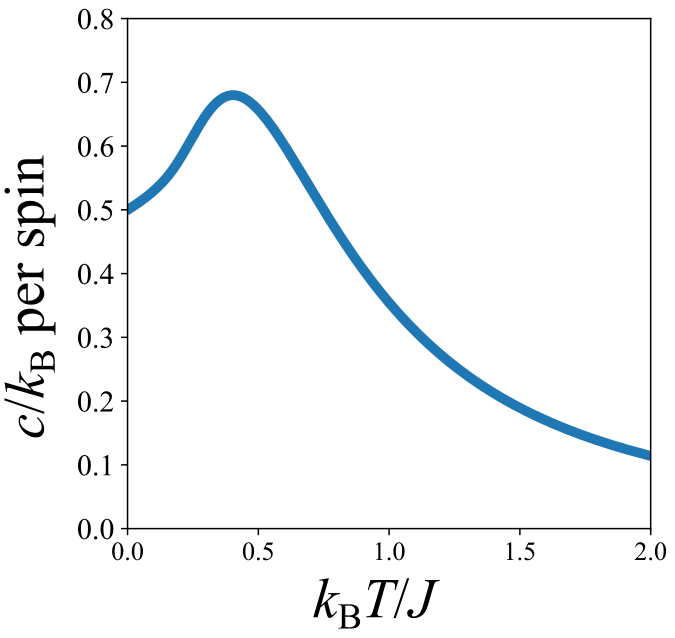
\includegraphics[scale=0.3]{1D_XY_Cv.png}
\caption{Exact specific heat of 1D XY model}
\end{figure}

The most physically interesting cases are the 2 dimensional and the 3 dimensional
ones and they will be discussed in details in the following sections.


\section{2D case}

Phase transitions are classified based on discontinuities of derivatives of the 
free energy, e.g. a ferromagnetic transition is a second-order phase transition 
because it is the magnetic susceptibility, the second derivative of the free energy
with respect of the magnitude of the external field, to be discontinous at the 
critical temperature while the magnetization, the first derivative, is continous.

The 2D case for the XY model is very peculiar because it can be shown to exhibit an
\emph{infinite-order} phase transition called a Kosterlitz-Thouless transition 
after the physicists that first studied it. \footnote{see 
\cite{Kosterlitz_1973}. Thouless and Kosterlitz were awarded the Nobel Prize in 
Physics in 2016 "for theoretical discoveries of topological phase transitions and 
topological phases of matter." 
\url{https://www.nobelprize.org/prizes/physics/2016/summary/}}

The Kosterlitz-Thouless transition consists of a transition between a quasi-ordered 
phase under the critical temperature with a correlation function with a powerlaw
decrease with distance and a disordered phase over the critical temperature with 
a correlation decreasing exponentially with the distance. These kind of order and
disorder states can be shown by identifing vortices in the system. Kosterlitz and 
Thouless gave the following thermodinamical argumentation to show the existence of such
transition. In the ground state at low temperatures all spins are in the same 
orientation and adding a single vortex will change the entropy of the system by
an amount $\Delta S = k_B \ln(L^2 / a^2)$ where $L$ is the system size, while $a$ 
is the radius of the vortex core. The change in internal energy of the system will
be instead $\Delta E = \pi J \ln(L/a)$. Then the amount of change of free energy will be:
$$ \Delta F = \Delta E - T \Delta S = (\pi J - 2 k_B T) \ln(L/a) $$
At high temperatures (for $\Delta F < 0$) in the thermodinamic limit the system 
will favor the formation of vortices, while viceversa at low temperatures
any vortex will try to annihilate with an antivortex to lower the system energy.
The critical temperature will be the one for which $\Delta F = 0$, so $T_c = \pi
J / 2 k_B$.

Theoritical and Monte Carlo simulation estimates of the critical temperature have
been attempted over the years reaching the well established value of $k_B T_c / J
\simeq 0.88$. Monte Carlo simulations allow also to visualize this kind of 
behaviour using a color map: mapping the spin angles with a colour using a 
continous and periodic color spectrum like a red-green-blue one, where the angle
spans in the interval $[-\pi, \pi)$, the formation of vortex-antivortex pairs can 
be shown at low temperatures as in figure~\ref{fig:kosterlitz}.
\footnote{source 
\url{https://upload.wikimedia.org/wikipedia/commons/7/77/XY_Vortices.svg}}

\begin{figure}[h]
\label{fig:kosterlitz}
\centering
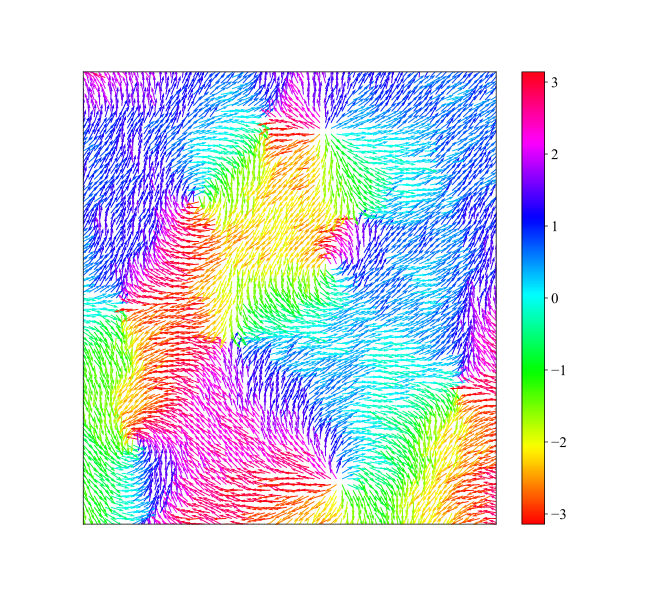
\includegraphics[scale=0.4]{kosterlitz.png}
\caption{Vortex-antivortex formations in 2D XY model at $k_B T / J = 0.4$}
\end{figure}
 

\section{3D case}

In the 3D case (and in higher dimensions) the XY model exhibits a 
ferromagnetic-paramagnetic transition at the critical temperature $k_B T_c / J 
\simeq 2.22$. From a physical point of view this transition plays a central role in
establishing the validity of the model because the values of the so called 
\emph{critical exponents} can be obtained via theoretical means, with quantum
field theory, by experiments and by Monte Carlo simulations.

Critical exponents are a very useful tool used in phase transition description.
They are employed to describe the behavior of physical quantities near the critical
temperature in a huge variety of different systems. They are used in 
\textit{n}-vector model descriptions because it is believed, on strong experimental 
basis, that they do not depend on the particulars of the physical system under
study but only on the following general properties:
\begin{itemize}
  \item the dimension of the system
  \item the dimension of the \emph{spins} considered
  \item the range of interaction
\end{itemize}

The critical exponents are usually denoted by a greek letter and usually the most
important ones are $\alpha$, $\beta$, $\gamma$ and $\delta$. Their meanings will
be explained in the next chapter. 
 
In 3 dimensions, critical exponents can be derived analytically in mean field
theory \footnote{see \url{https://en.wikipedia.org/wiki/Mean-field_theory}}
and experimentally by studying easy-plane magnets and liquid \ce{^{4}He}.

